%%%%%%%%%%%%%%%%%%%%%%%%%%%%%%%%%%%%%%%%%
% Beamer Presentation
% LaTeX Template
% Version 1.0 (10/11/12)
%
% This template has been downloaded from:
% http://www.LaTeXTemplates.com
%
% License:
% CC BY-NC-SA 3.0 (http://creativecommons.org/licenses/by-nc-sa/3.0/)
%
%%%%%%%%%%%%%%%%%%%%%%%%%%%%%%%%%%%%%%%%%

%----------------------------------------------------------------------------------------
%	PACKAGES AND THEMES
%----------------------------------------------------------------------------------------

\documentclass{beamer}

\mode<presentation> {

% The Beamer class comes with a number of default slide themes
% which change the colors and layouts of slides. Below this is a list
% of all the themes, uncomment each in turn to see what they look like.

%\usetheme{default}
%\usetheme{AnnArbor}
%\usetheme{Antibes}
%\usetheme{Bergen}
%\usetheme{Berkeley}
%\usetheme{Berlin}
%\usetheme{Boadilla}
%\usetheme{CambridgeUS}
%\usetheme{Copenhagen}
%\usetheme{Darmstadt}
%\usetheme{Dresden}
%\usetheme{Frankfurt}
%\usetheme{Goettingen}
%\usetheme{Hannover}
%\usetheme{Ilmenau}
%\usetheme{JuanLesPins}
%\usetheme{Luebeck}
%\usetheme{Madrid}
%\usetheme{Malmoe}
%\usetheme{Marburg}
%\usetheme{Montpellier}
%\usetheme{PaloAlto}
%\usetheme{Pittsburgh}
%\usetheme{Rochester}
%\usetheme{Singapore}
\usetheme{Szeged}
%\usetheme{Warsaw}

% As well as themes, the Beamer class has a number of color themes
% for any slide theme. Uncomment each of these in turn to see how it
% changes the colors of your current slide theme.

%\usecolortheme{albatross}
\usecolortheme{beaver}
%\usecolortheme{beetle}
%\usecolortheme{crane}
%\usecolortheme{dolphin}
%\usecolortheme{dove}
%\usecolortheme{fly}
%\usecolortheme{lily}
%\usecolortheme{orchid}
%\usecolortheme{rose}
%\usecolortheme{seagull}
%\usecolortheme{seahorse}
%\usecolortheme{whale}
%\usecolortheme{wolverine}

%\setbeamertemplate{footline} % To remove the footer line in all slides uncomment this line
%\setbeamertemplate{footline}[page number] % To replace the footer line in all slides with a simple slide count uncomment this line

%\setbeamertemplate{navigation symbols}{} % To remove the navigation symbols from the bottom of all slides uncomment this line
}

\usepackage{graphicx} % Allows including images
\usepackage{booktabs} % Allows the use of \toprule, \midrule and \bottomrule in tables
\usepackage{hyperref}
\usepackage{xcolor}

%----------------------------------------------------------------------------------------
%	TITLE PAGE
%----------------------------------------------------------------------------------------

\title[L0 Backgrounds]{L0 Upgrade Background Study} % The short title appears at the bottom of every slide, the full title is only on the title page

\author{Matt Solt} % Your name
\institute[Stanford] % Your institution as it will appear on the bottom of every slide, may be shorthand to save space
{
SLAC National Accelerator Laboratory \\ % Your institution for the title page
\medskip
\textit{mrsolt@slac.stanford.edu} % Your email address
}
\date{\today} % Date, can be changed to a custom date

\begin{document}

\begin{frame}
\titlepage % Print the title page as the first slide
\end{frame}

%----------------------------------------------------------------------------------------
%	PRESENTATION SLIDES
%----------------------------------------------------------------------------------------

%------------------------------------------------
%\section{First Section} % Sections can be created in order to organize your presentation into discrete blocks, all sections and subsections are automatically printed in the table of contents as an overview of the talk
%------------------------------------------------

%\subsection{Subsection Example} % A subsection can be created just before a set of slides with a common theme to further break down your presentation into chunks

\begin{frame}
\frametitle{Introduction}
\begin{itemize}
\item L0 upgrade simulations include additional tracking layer (layer 0) between target and current first layer and moving current L2 and L3 towards beam by 0.8 mm
\item Resolved issues in the simulation that affected backgrounds (but had little affect on everything else)
\begin{itemize}
\item L0 shifted due to not taking the beam rotation into account
\item Incorrect charge sharing matrix used for L0 strips (no intermediate strips unlike other layers)
\item MC wabs had generator level cut at 15 mrad and L2 and L3 now dip below that (now set at 5 mrad)
\end{itemize}
\item Basic background studies and trigger rates are reported using wab-beam-tri MC (i.e. beam)
\end{itemize}

\end{frame}

%------------------------------------------------

\begin{frame}
\frametitle{Cross Section Comparison}
\begin{itemize}
\item Occupancies defined using 8 ns time windows
\item $Cluster Occupancy = \frac{Strip Occupancy}{Cluster Size Average}$ (Cluster size average is 1.1 for L0 and 1.5 for all other layers)
\end{itemize}
\begin{figure}
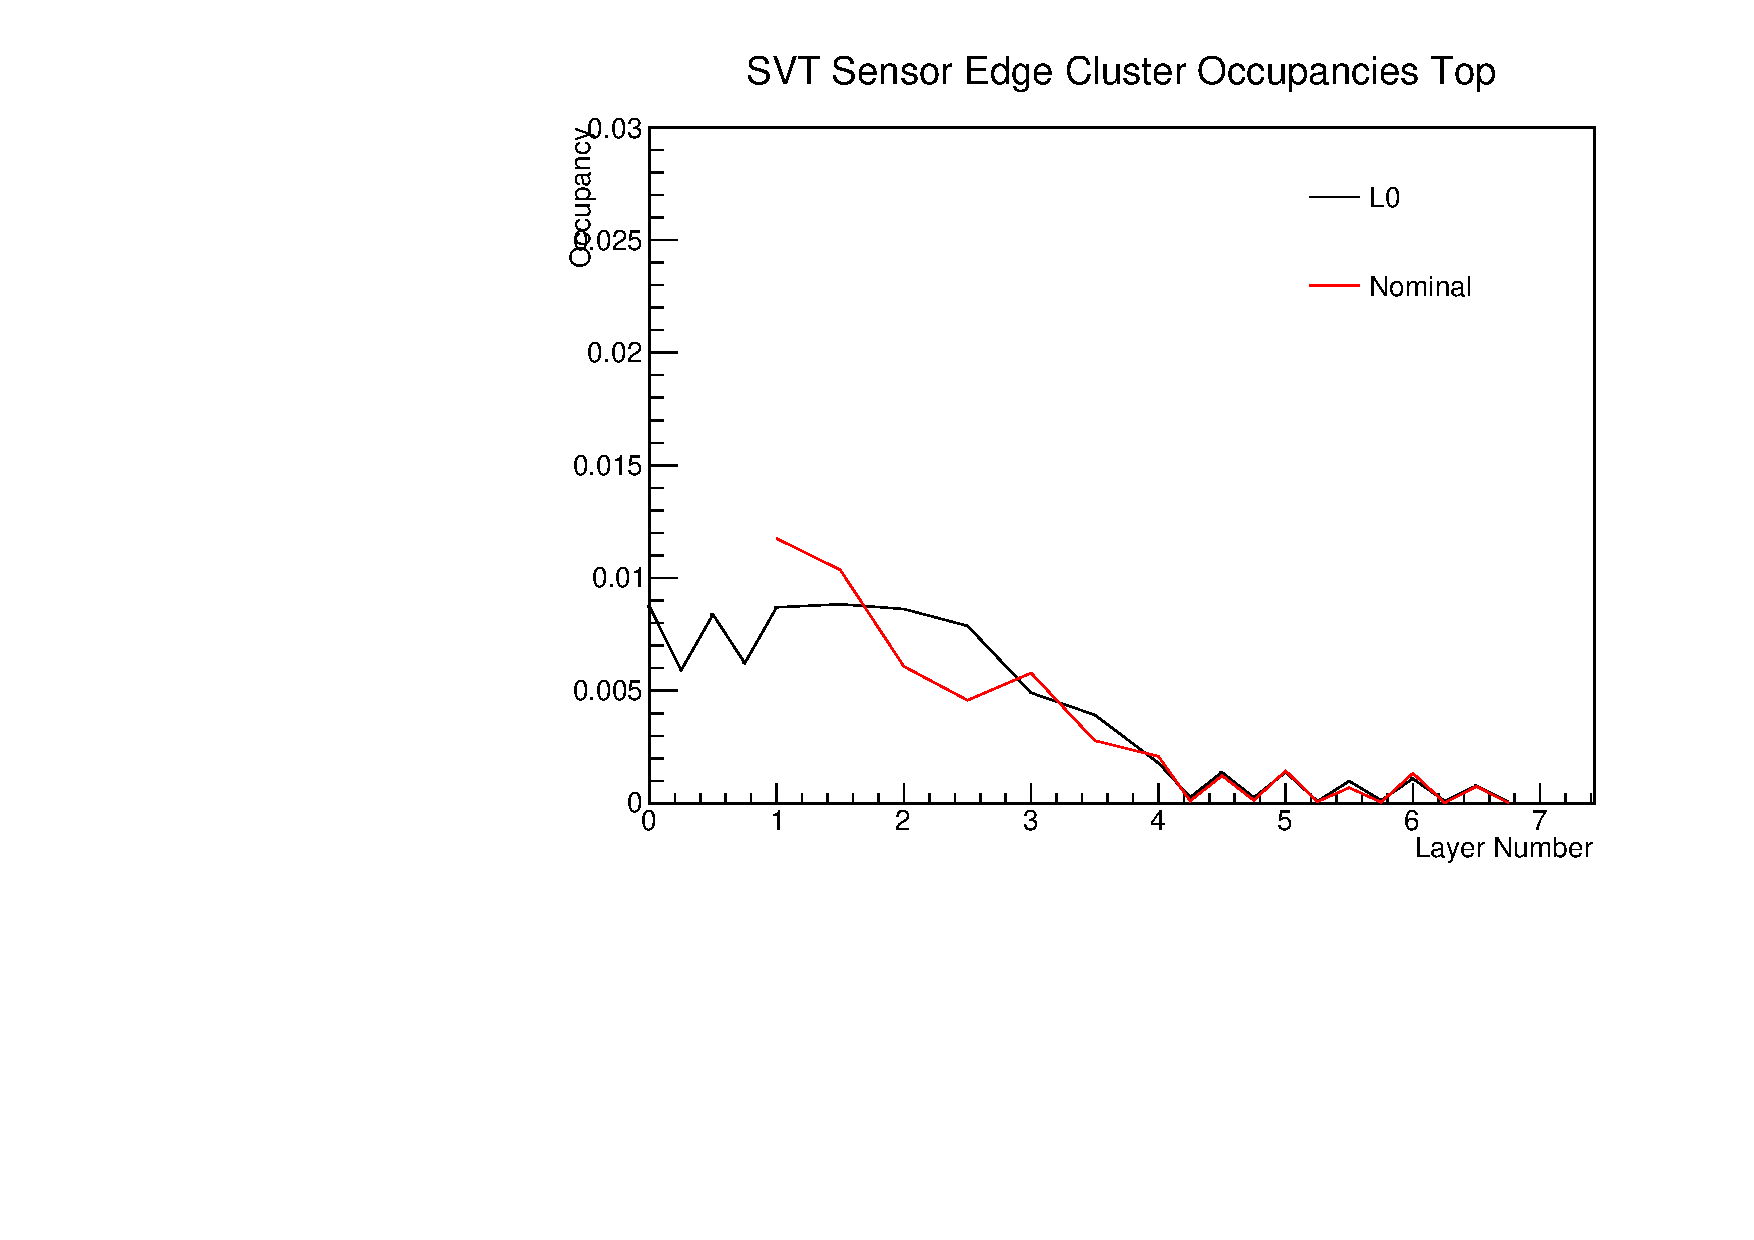
\includegraphics[width=0.55\linewidth]{figs/occupancy_top.pdf}
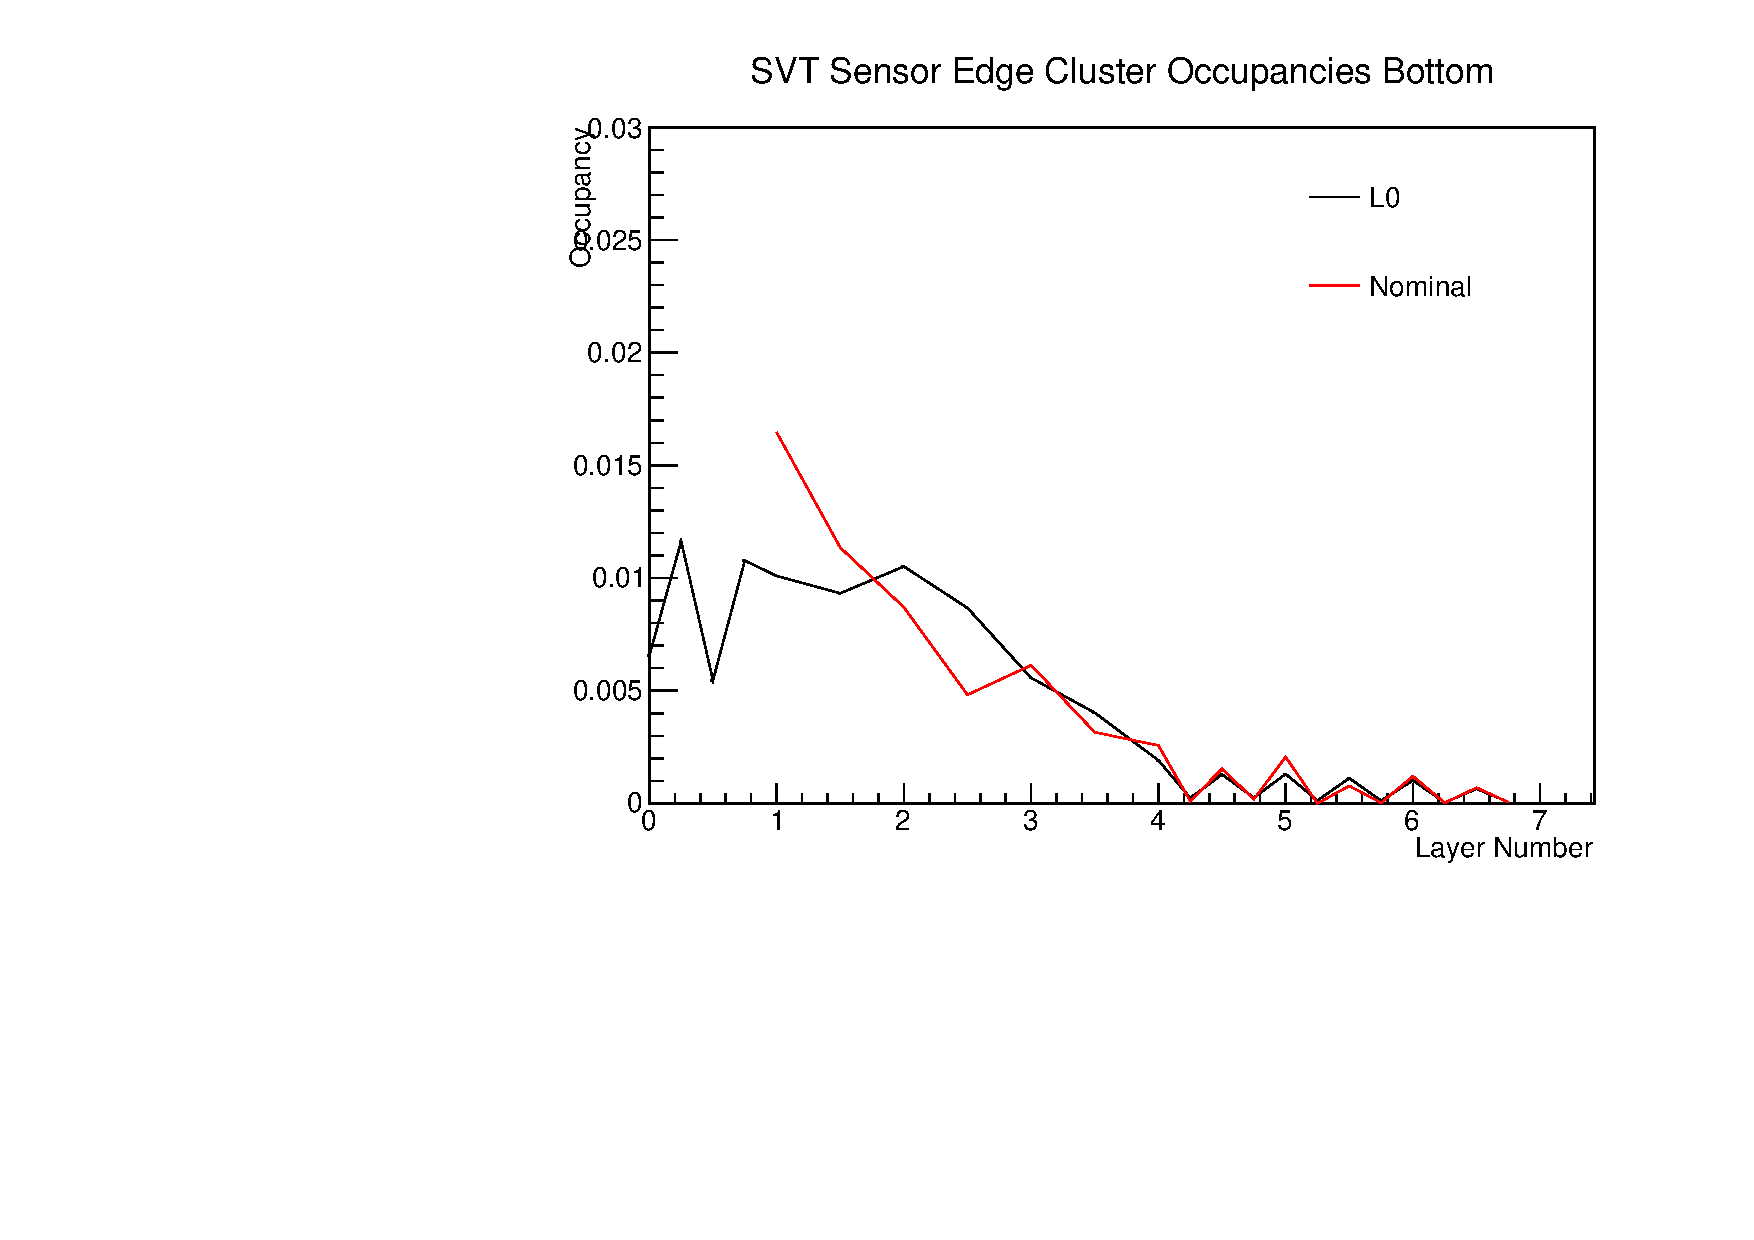
\includegraphics[width=0.55\linewidth]{figs/occupancy_bot.pdf}
\end{figure}

\end{frame}

%------------------------------------------------

\begin{frame}
\frametitle{Trigger Rates}
\begin{itemize}
\item L0 trigger rate is \textbf{\textit{31.2 kHz}}
\item Nominal trigger rate is \textbf{\textit{23.0 kHz}}
\item Detailed reasons for the increase trigger rates are to be explored
\begin{itemize}
\item Plot trigger rate as function of cluster position in Ecal. Separate these by charged particles and photons
\item Plot of $z$ origin of particles that generate trigger clusters. Separate by charged and neutral particles
\end{itemize}
\end{itemize}

\end{frame}

%------------------------------------------------

\begin{frame}
\frametitle{Degraded Vertex Resolution}
\begin{itemize}
\item Comparison of vertex resolution for nominal detector and L0 detector where L0 is not used for tracking (resolution degrades slightly due to multiple scattering)
\end{itemize}
\begin{figure}
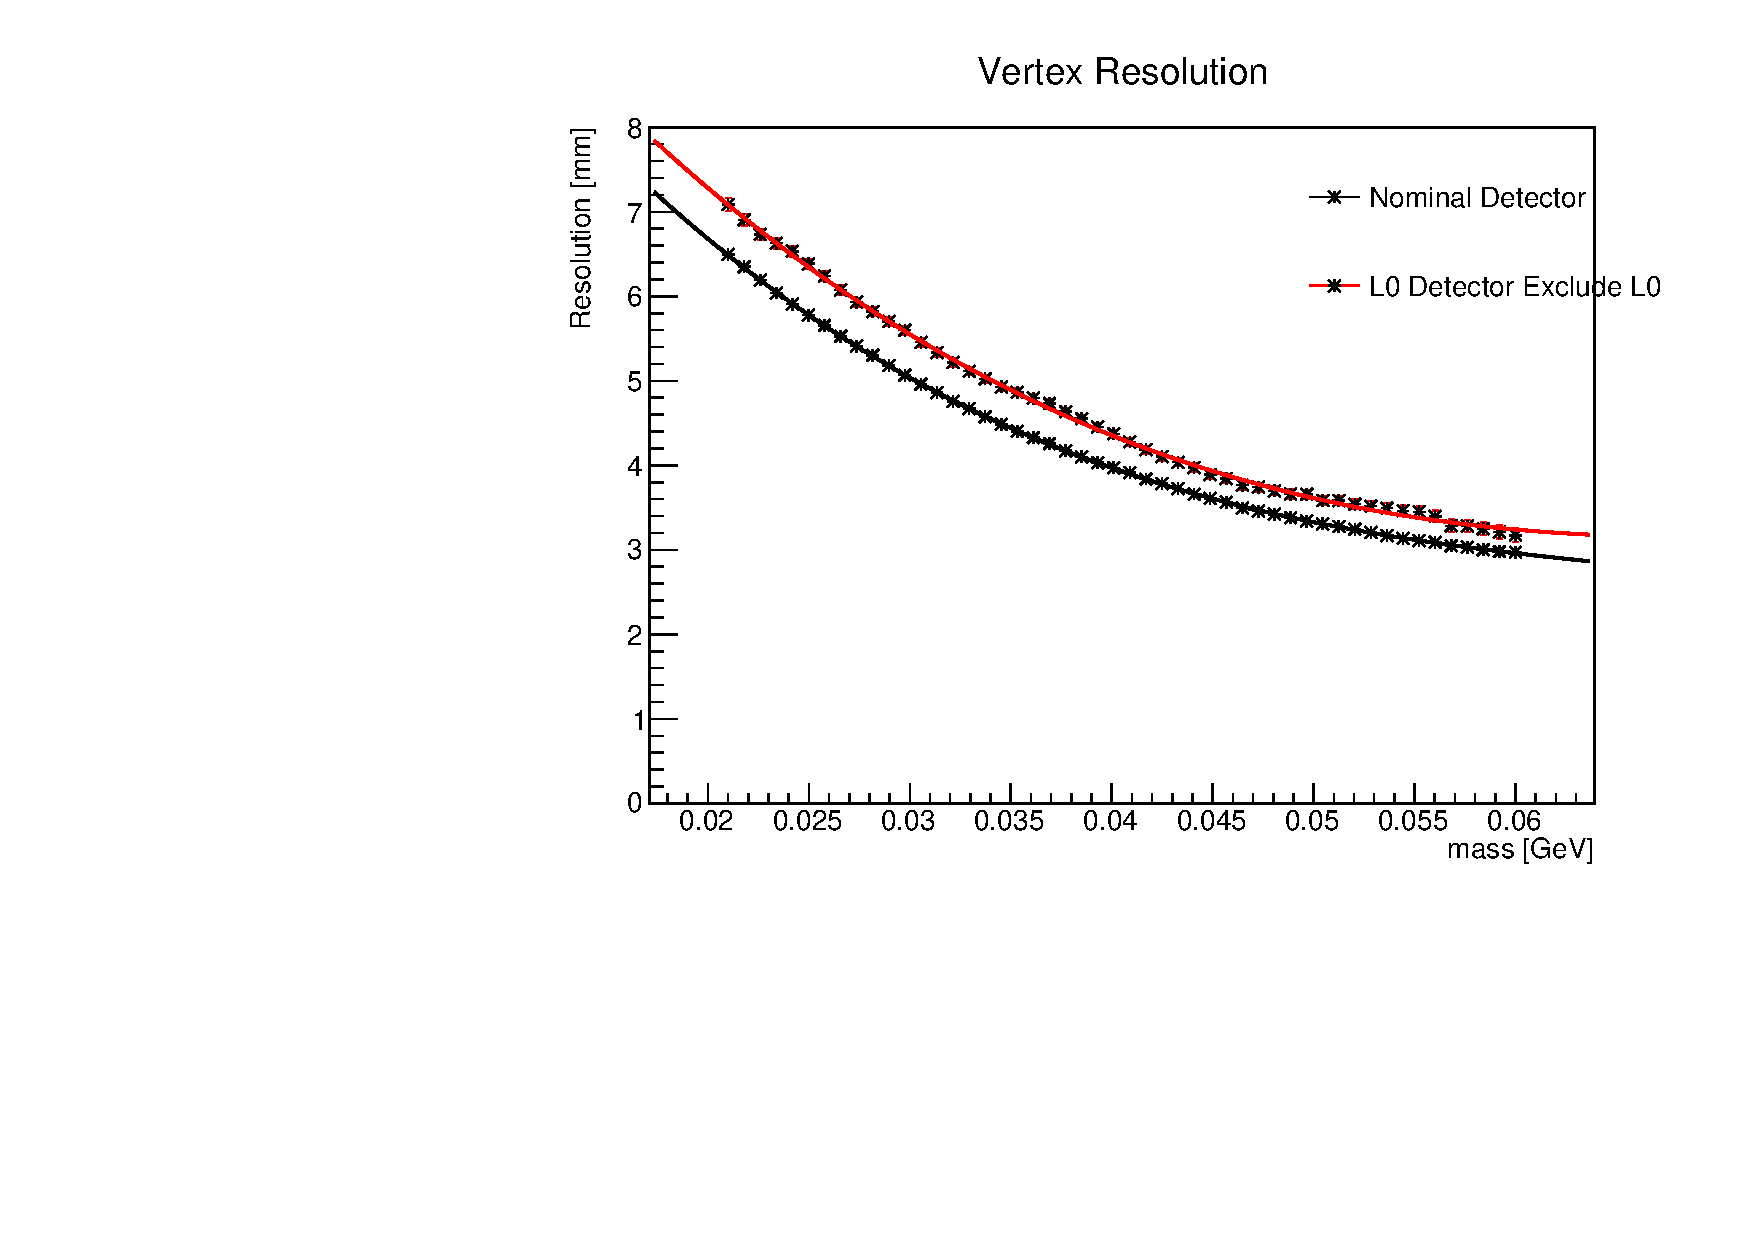
\includegraphics[width=0.65\linewidth]{figs/VZ_Resolution.pdf}
\end{figure}

\end{frame}

%------------------------------------------------

\end{document} 
